%%%%%%%%%%%%%%%%%%%%%%%
%%% Document Set up %%%
%%%%%%%%%%%%%%%%%%%%%%%

\documentclass[11pt]{amsart}


% you can add extra packages if you need them
\usepackage{amsfonts, amssymb, amscd, amsmath, amsthm, enumerate, verbatim, calc, 
thumbpdf, mathrsfs, graphicx, multicol, tabu, tikz}

\usetikzlibrary{snakes}
\tikzstyle{printersafe}=[snake=snake,segment amplitude=0 pt]

\setlength{\oddsidemargin}{0.25in}  % please do not change
\setlength{\evensidemargin}{0.25in}  % please do not change
\setlength{\marginparwidth}{0in}  % please do not change
\setlength{\marginparsep}{0in}  % please do not change
\setlength{\marginparpush}{0in}  % please do not change
\setlength{\topmargin}{0in}  % please do not change
\setlength{\footskip}{.3in}  % please do not change
\setlength{\textheight}{8.75in}  % please do not change
\setlength{\textwidth}{6in}  % please do not change
\setlength{\parskip}{4pt}  % please do not change


\theoremstyle{plain}  % default
\newtheorem{thm}{Theorem}[section]
\newtheorem{lem}[thm]{Lemma}
\newtheorem{cor}[thm]{Corollary}
\newtheorem{prop}[thm]{Proposition}
\newtheorem{mythm}[thm]{My Great Result}

\theoremstyle{definition}
\newtheorem{defin}[thm]{{Definition}}
\newtheorem{ex}[thm]{Example}

\theoremstyle{remark}
\newtheorem{rem}[thm]{Remark}
\newtheorem*{note}{Note}
\newtheorem{case}{Case}

\numberwithin{equation}{thm}

\newcommand{\dims}{\operatorname{dims}}
\newcommand{\rank}{\operatorname{rank}}

\DeclareMathOperator{\lcm}{lcm}

\usetikzlibrary{arrows}



%%%%%%%%%%%%%%%%%%%%%%%%%%%%%%%%%
%%% Document Meta Information %%%
%%%%%%%%%%%%%%%%%%%%%%%%%%%%%%%%%


\begin{document}


\title[Investigation of resolving sets and metric dimension]{Investigation of resolving sets and metric dimension}
\author[K.~ R. Ryan]{Kyle Ryan}
\thanks{Advisors: Trevor McGuire, Warren Shreve}

\address{Department of Mathematics 2750\\ North Dakota State University\\PO BOX 6050\\ Fargo, ND 58108-6050\\ USA}

\email{kyleryanmn@gmail.com, trevor.mcguire@ndsu.edu, warren.shreve@ndsu.edu}





\maketitle
% \setcounter{page}{***} % Please do not change this line


\begin{abstract}
        For any graph G it is possible to describe each of its vertices uniquely with respect to an ordered subset of vertices of G called a resolving set.
    In this paper we will investigate properties associated with minimal resolving sets, known as bases and conditions under which changing G affects its bases. 
\end{abstract}

%%%%%%%%%%%%%%%%%%%%
%%% Introduction %%%
%%%%%%%%%%%%%%%%%%%%

\section{introduction}

    %The basics of what you're doing: relevant tools, defs techniques etc%
    For this investigation we will begin with several basic definitions that might not be part of a typical introduction to graph theory.

 \begin{defin}[Representation of vertex(with respect to W)]:\\
    For an ordered subset $W=(w_1, w_2, ...)$ of vertices in $G$, the representation of a vertex $v \in G$ with respect to $W$ denoted $rep(v/W)$ is:
  \begin{align*}
  rep(v/W)=(d(v,w_1), d(v,w_2), ...)
  \end{align*}
 \end{defin}
    
 \begin{defin}[Resolving Set]:\\
  An ordered subset $W \subset V(G)$ is called a resolving set of G if for all $v_1, v_2 \in V(G)$: 
  \begin{align*}
  rep(v_1/W) \neq  rep(v_2/W)
  \end{align*}
 \end{defin}
 
 \begin{defin}[Basis of a graph]:\\
  A resolving set $W$ of $G$ is called a $basis\ of\ G$ if for any other resolving set $H$ of $G$, 
  \begin{align*}
   |H| \geq |W|
  \end{align*}

 \end{defin}
 
 \begin{defin}[Metric Dimension]:\\
  The metric dimension of a graph $G$ denoted $MD(G)$ is the order of any basis for $G$.
 \end{defin}


Finding the metric dimension or any basis for a graph is currently considered to be an NP-Hard problem. 
Metric dimension is known for some subsets of graphs which will be discussed later, but in general it is very difficult or simply time consuming to determine.
The intent of this paper is to investigate whether there is a set of graphs for which having a known metric dimension allows us to determine metric dimension after adding or removing an edge.
Furthermore we will attempt to investigate what properties of these graphs make it possible to determine metric dimension for them after adding or removing an edge.
\begin{ex}
 The path graph $P_3$ has a metric dimension of 1. Simply calling $W$ the set containing one leaf node of $P_3$ is sufficient to construct a basis for $P_3$.
 By adding any edge to $P_3$, $P_3$ becomes $K_3$ which has a metric dimension of 2.
\end{ex}
 \begin{tikzpicture}[>=stealth',shorten >=1pt,auto,node distance=3cm,
                    thick,main node/.style={circle,draw,font=\sffamily\Large\bfseries}]
  \node[main node] (1) {x};
  \node[main node] (2) [right of=1] {};
  \node[main node] (3) [right of=2] {x};
  \node[main node] (4) [right of=3] {};
  \node[main node] (5) [above of=4] {y};
  \path[thick]
    (1)	edge (2)
    (3) edge (4)
    (4) edge (5)
    (3) edge [dashed, printersafe] (5);
\end{tikzpicture}

%%%%%%%%%%%%%%%%%%%%%%%%%%%%%%%%%%%%%%%%%%%%%%%%%%%%%%%%
%%%%%%%       SECTION 1, B-Encodings          %%%%%%%%%%
%%%%%%%%%%%%%%%%%%%%%%%%%%%%%%%%%%%%%%%%%%%%%%%%%%%%%%%%
\section{encodability of graphs with respect to their bases}


  \begin{defin}[Representation set of a graph]%:\\
  The representation set of a graph with respect to a basis $W$ is the set $H=\{r(v/W)\mid v\in G\}$.   
  \end{defin}

  \begin{defin}[Unique Encoding]%:\\
   If we can construct a graph $G$ from its representation set $H$ by connecting vertices in $G$ 
   if their representations differ by no more than 1 in each place then we say that $G$ is uniquely encoded by $H$.
   Furthermore we say that $G$ is uniquely encodeable with respect to its basis $W$ or $G$ is enccodable under $W$.
  \end{defin}

\begin{lem}
A graph $G$ is encodable under $W$ if and only if for all nonadjacent $\ v_1,\ v_2\in G$ there exists $w \in W$ such that:
\begin{align*}
| d(v_1,w)-d(v_2,w)| > 1 
\end{align*}
\end{lem}
\begin{proof}
Let $G$ be a graph with basis $W$. Let $R$ be the representation set of $G$ with respect to $W$. 
Assume that for some pair of non adjacent vertices $v_1,\ v_2\ \in G$, $\ \exists\ w \in W$ such that $\left| d(v_1,w)-d(v_2,w)\right| \leq 1$.
If we construct a graph $H$ from $R$ following the encoding scheme described above, $v_1,\ v_2$ will be adjacent in $H$. 
Then $H \neq G$ and so $G$ is not encodable under $W$. If for all nonadjacent $\ v_1,\ v_2\in G$ there exists $w \in W$ such that 
$|d(v_1,w)-d(v_2,w)| > 1$, no pair of nonadjacent vertices will be adjacent in $H$. For every pair of adjacent vertices $v_1,\ v_2$ in $G$ and $w\in W$,  
$\left| d(v_1,w)-d(v_2,w)\right| \leq 1$ 
and so they will be adjacent in $H$. Thus $G$ is encodable under $W$ if and only if for all nonadjacent $\ v_1,\ v_2\in G$ there exists $w \in W$ such that $|d(v_1,w)-d(v_2,w)| > 1$.
\end{proof}

\begin{ex}
Observe the following\\

\begin{tikzpicture}[>=stealth',shorten >=1pt,auto,node distance=3cm,
                    thick,main node/.style={circle,draw,font=\sffamily\Large\bfseries}]
\node[main node] (1) {x};
\node[main node] (2) [above right of=1] {};
\node[main node] (3) [above left of=1] {};
\node[main node] (4) [above of=2] {y};
\node[main node] (5) [above of=3] {};

\path[thick]
  (1) edge (2)
      edge (3)
  (2) edge (3)
      edge (4)
  (3) edge (5);

\node[main node] (8) [right of=2] {x};
\node[main node] (6) [below right of=8]{};
\node[main node] (7) [above right of=6] {};
\node[main node] (9) [above of=7] {y};
\node[main node] (10) [above of=8] {};

\path[thick]
  (6) edge (7)
      edge (8)
      edge [dashed, printersafe] (10)
  (7) edge (8)
      edge (9)
  (8) edge (10);
  
\end{tikzpicture}

\begin{tikzpicture}[>=stealth',shorten >=1pt,auto,node distance=3cm,
                    thick,main node/.style={circle,draw,font=\sffamily\Large\bfseries}]
\node[main node] (1) {x};
\node[main node] (2) [above right of=1] {};
\node[main node] (3) [above left of=1] {y};
\node[main node] (4) [above of=2] {};
\node[main node] (5) [above of=3] {};

\path[thick]
  (1) edge (2)
      edge (3)
  (2) edge (3)
      edge (4)
  (3) edge (5)
  (5) edge [dashed, printersafe] (2)
      edge [dashed, printersafe] (4);

\node[main node] (8) [right of=2] {x};
\node[main node] (6) [below right of=8]{};
\node[main node] (7) [above right of=6] {y};
\node[main node] (9) [above of=7] {};
\node[main node] (10) [above of=8] {};

\path[thick]
  (6) edge (7)
      edge (8)
      edge [dashed, printersafe] (9)
      edge [dashed, printersafe] (10)
  (7) edge (8)
      edge (9)
  (8) edge (10)
  (9) edge [dashed, printersafe] (10);
\end{tikzpicture}
\\
The bull graph pictured above has basis size 2. There are 4 possible bases for it up to isomorphism but is W-encodable only under one of them.
For the other 3 bases it is possible to add edges (shown dotted) without affecting $r(v/W)$ for any $v \in G$.

\end{ex}


\section{Upper and Lower Bounds on Metric Dimension}

%\begin{lem}
% let $G$ be a unicyclic graph. Let $L$ be the cycle in $G$. Let $l$ be the number of $deg > 2$ vertices of $L$. 
% Let $H = G-L$. Then:
% \begin{align*}
% MD(G) &\leq 2 + MD(H) -l\ if\ L\ is\ an\ odd\ cycle\\
% MD(G) &\leq 3 + MD(H) -l\ if\ L\ is\ an\ even\ cycle
% \end{align*}
%\end{lem}
%\begin{proof}
%Odd case: \\
%Even case: \\
%  I am still working on tidying up the proof of this. I will add it when it is ready for print.
%\end{proof}

%\begin{lem}
% Let $G$ be a graph with a bridge $(u,v)$ s.t. $G-(u,v)$ has components $H_1, H_2$ such that $H_1$ 
% has at least one degree $>$ 2 vertex. Then for any basis $W$ of $G$, $W\nsubseteq H_2$.
%\end{lem}
%\begin{proof}
 
%\end{proof}
\begin{lem}
 Let $G$ be a graph with a cut vertex $v$ and resolving set $W$. Let $H$ be a component of $G-v$. 
 If $G-v$ has more than two components or if for any component $L$ of $G-v$, $L$ is not a path, then $W\nsubseteq H$.
\end{lem}
\begin{proof}
 Suppose that $W \subset H$. 
 Let $v$ be a cut vertex of $G$ such that $G-v$ has more than 2 components. Since $W \subset H$, the path from any vertex not in $H$ to any element of $W$ must pass through $v$.
 Then there exist vertices $u_1,\ u_2$ adjacent to $v$ such that $d(u_1, w_i) = d(u_2, w_i) = d(v, w_i) + 1$ for all $w_i \in W$.
 In this case, $r(u_1/W) = r(u_2/W)$. Then $W$ cannot be not a resolving set for $G$.\\
 We can show without loss of generality that the same is true for any cut vertex $v$ whenever some component of $G-v$ other than $H$ is not path.\\
 Observe that if $G$ is not a path it contains at least one $deg > 2$ vertex. 
 Let $l$ be a $deg > 2$ vertex in $G$ such that for all$u_i$ such that $deg(u_i)>2, d(u_i, v) \geq d(l, v)$. 
 Then by the same argument as above we see there are 2 adjacent vertices with the same representation and again $W$ cannot be a resolving set of $G$.
 \end{proof}

\begin{lem}[Bridge Subdivision Lemma]
 %$i:$ If only $H$ contains a basis element then $MD(G)\leq MD(G')$.\\
 %$ii:$ If $H$ and $S$ both contain basis elements then $MD(G') = MD(G)$
 If $G$ is a graph with a bridge $L$ separating two non path subraphs which are only connected through $L$ 
 then subdivision of $L$ leaves the bases of $G$ unchanged.  
\end{lem}
\begin{proof}$\ $\\
 %$i)$ Since $S'$ contains no basis elements, $S'$ must be a path.\\
 %We can contract $(u,e)$ to $u$ to construct $G$ from $G'$.\\
 %Then for each element $v_{s'}$ of $S'$, $rep(v_s/W) = rep(v_s/W) - (1,...,1)$ \\\\
 %$ii)$ Suppose that $MD(G') > MD(G)$, this can only be true if for some $u_h \in H$, $v_s\in S$ 
 Let $G$ be a graph with a bridge $(u,v)$.\\
 Let $H, S$ be the largest connected induced subgraphs of $G$ such that\\ $ u\in H,\ v\notin H, v\in S,\ u\notin S$.\\
 Let $L$ be the $uv$ path separating $H$ and $S$.\\
 Let $W$ be a basis of $G$.\\
 Let $G', H', S', L', W'$ be the same objects described above after subdivision of $(u,v)$ with vertex $e$ and the additional constraint that
 $e \notin H' \cup S'$.\\
 
 $i)$%If H and S both contain basis elements in $G$, then $W = W'$\\
 If $H$ and $S$ both contain basis elements in $G$, then $W$ resolves $G'$.\\ 
 Suppose that for some basis $W$ of $G$, $W$ does not resolve $G'$, this can only be true if for some $u_h \in H$, $v_s\in S$
\begin{align*}
 r(u_h/W) + (\underbrace{0,\dots}_{n},1,\dots) = r(v_s/W) + (\underbrace{1,\dots}_{n},0,\dots),
\end{align*}
where the first n elements of each representation correspond to the distances from elements of $W_h$ up to rearrangement.\\
Suppose that such a pair of vertices does exist. Then for all $w_h\in W_H \subset H$,\\ $d(v_s, w_h)<d(u_h, w_h)$.\\
Every $v_sw_h$ path for all $w_h$ passes through $L$. Then $d(v_s, w_h)=d(v_s, u)+ d(u, w_h)$. 
By the triangle inequality, $d(u_h, w_h) \leq d(u_h, u) + d(u, w_h)$ for all $u_h$ in $H$.
Then $d(v_s, u)<d(u_h,u)$ and consequently $d(v_s, e)<d(u_h, e)$.\\
Without loss of generality we can show that because for all $w_s\in W_S\subset S$, $d(u_h, w_s)<d(v_s, w_s)$ we must have
$d(u_h, e)<d(v_s,e)$. This is a contradiction. Then such a pair of vertices cannot possibly exist and so we have $W$ resolves $G'$.\\
$ii)$If $H'$ and $S'$ both contain basis elements in $G'$, then $W'$ resolves $G'$.\\ 
In this case we see that we must have a pair of vertices $u_h \in H'$, $v_s\in S'$ such that
\begin{align*}
 r(u_h/W') + (\underbrace{1,\dots}_{n},0,\dots) = r(v_s/W') + (\underbrace{0,\dots}_{n},1,\dots),
\end{align*}
where the first n elements of each representation correspond to the distances from elements of $W'_h$ up to rearrangement. 
Again we will suppose that such a pair of vertices exists.\\ 
Then we can see that for basis elements in $H'$:
\begin{align*}
d(u_h, w_h) + 1 &= d(v_s,w_h)\\
d(u_h, u) + d(u, w_h) + 1 &= d(v_s, u) + d(u, w_h)\\
d(u_h, u) + 1 &= d(v_s, u)\\
d(u_h, u) + 1 &> d(v_s, u) - 1\\
d(u_h, u) + d(u, e) &> d(v_s, u) - d(u, e)\\
d(u_h, e) &> d(v_s, e).
\end{align*}
Without loss of generality, we consider basis elements in $S'$ and notice:
\begin{align*}
 d(v_s, e) &> d(u_h, e).
\end{align*}
Then $d(v_s, e) >< d(u_h, e)$, a clear contradiction.\\
Thus $W'$ resolves $G$, and so $W = W'$.\\ \\
%$iii)$ If only $H$ contains a basis element then
%From part $ii$ above we see that if $H'$ and $S'$ both contain basis elements then $H$
\end{proof}


%\begin{lem}
% Let $G$ be any graph. Let $H$ be the graph obtained by edge contractions on $G$. 
% If only the number of degree 2 vertices is changed, 
%\end{lem}
%\begin{proof}
 
%\end{proof}






%%%%%%%%%%%%%%%%%%%%%%%%%%%%%%%%
%%% References and Citations %%%
%%%%%%%%%%%%%%%%%%%%%%%%%%%%%%%%
\cite{Chartrand:2010:GDF:1941879}
\nocite{*}
\bibliographystyle{plain}
\bibliography{mybib}  % add references to the list of references saved in the file mybib.bib


\end{document}
